\documentclass[11pt,twoside]{scrartcl}
\usepackage{mdas}
% \usepackage[sexy, fancy, hints]{evan}
\begin{document}
\title{How to Use Tikz}
% If you contribute to the handout, put your name in comment here

\author{manojdas1@gmail.com}
\org{Manoj Latex Notes}
\date{\today}

\maketitle

\begin{abstract}
    Usage examples for Tikz. 
\end{abstract}

\section{Examples}

\subsection{Bipartite Graph}
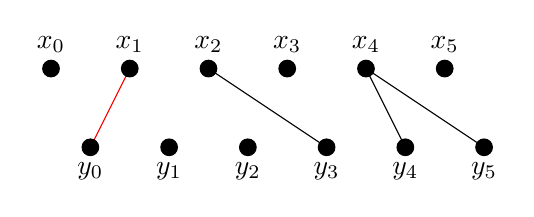
\begin{tikzpicture}
    \draw[red] (.5,0) -- (1,1);
    \draw (2,1) -- (3.5,0);
    \draw (4,1) -- (4.5,0);
    \draw (4,1) -- (5.5,0);
    \foreach \x in {0,...,5}
    {
        % \draw (\x,0) circle (3pt);

        \filldraw (\x, 1) circle (3pt);
        \path node at (\x, 1.3) {$x_{\x}$};
        \filldraw (\x + 0.5, 0) circle (3pt);
        \path node at (\x + 0.5, -.3) {$y_{\x}$};
    }
\end{tikzpicture}

\subsection{Markov Chain}
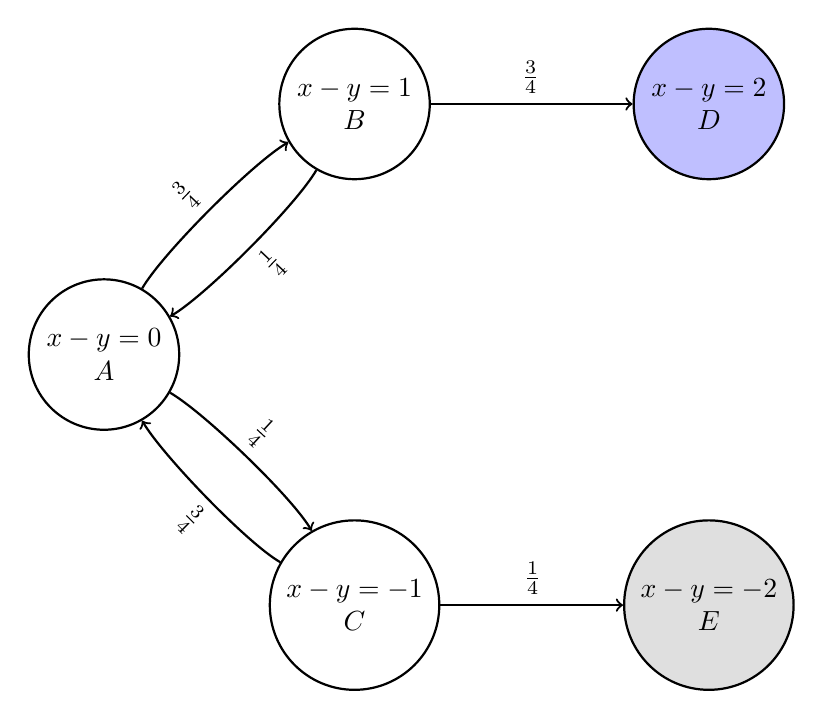
\begin{tikzpicture}[node distance={45mm}, thick, main/.style = {draw, circle}] 
    \node[main, align=center] (1) {$x-y=0$\\$A$}; 
    \node[main, align=center] (2) [above right of=1] {$x-y=1$\\$B$}; 
    \node[main, align=center] (3) [below right of=1] {$x-y=-1$\\$C$}; 
    \node[main, align=center] (4) [right of=2, fill=blue!25] {$x-y=2$\\$D$}; 
    \node[main, align=center] (5) [right of=3, fill=gray!25] {$x-y=-2$\\$E$}; 
    \draw[->] (1) to [out=60, in=210, looseness=.5] node[midway, above right, sloped, pos=0.4] {$\frac{3}{4}$}(2); 
    \draw[->] (2) to [out=240, in=30, looseness=.5] node[midway, below left, sloped, pos=0.4] {$\frac{1}{4}$}(1); 
    \draw[->] (1) to [out=-30, in=120, looseness=.5] node[midway, above right, sloped, pos=0.4] {$\frac{1}{4}$}(3); 
    \draw[->] (3) to [out=150, in=-60, looseness=.5] node[midway, below left, sloped, pos=0.4] {$\frac{3}{4}$}(1); 

    \draw[->] (2) to node[midway, above right, sloped, pos=0.4] {$\frac{3}{4}$}(4); 
    % \draw[->] (4) to [out=195, in=-15, looseness=.5] node[midway, above right, sloped, pos=0.6] {+2}(2); 

    \draw[->] (3) to  node[midway, above right, sloped, pos=0.4] {$\frac{1}{4}$}(5); 
    % \draw[->] (5) to [out=195, in=-15, looseness=.5] node[midway, above right, sloped, pos=0.6] {+2}(3); 
    % \draw[->] (6) -- node[midway, above right, sloped, pos=1] {+1} (4); 
\end{tikzpicture} 

\section{Trees}
\begin{figure}[h]
    \begin{tikzpicture}
        [
        level 1/.style = {red, sibling distance = 2cm},
        level 2/.style = {blue, sibling distance = 2cm},
        level 3/.style = {red, sibling distance = 2cm},
        level 4/.style = {blue, sibling distance = 1.5cm},
        level 5/.style = {red, sibling distance = 2cm},
        level 6/.style = {blue, sibling distance = 2cm},
        level 7/.style = {red, sibling distance = 2cm},    
        ]
        \tikzstyle{hollow node}=[circle,draw,inner sep=2.5]
        \tikzstyle{solid node}=[circle,draw,inner sep=2.5,fill=black]
        \tikzstyle{win node}=[rectangle,draw=blue,inner sep=2.5]
    
        \node[blue]{(10)}
        child{node[]{(8,4)} 
            child{node[win node]{(4,4)}}
            child{node[win node]{(5,5)}}
            child{node[]{(6,4)}
                child{node[]{(5,2)}
                    child{node[win node]{(3,3)}}
                    child{node[]{(4,2)}
                        child{node[]{(3,2)}
                            child{node[win node]{(2,2)}}
                            child{node[win node]{(1,1)}}
                        }
                    }    
                }
            }
            child{node[right=5.5cm]{(7,2)}
                child{node[]{(5,4)}
                    child{node[]{(4,2)}
                        child{node[]{(3,2)}
                            child{node[win node]{(2,2)}}
                            child{node[win node]{(1,1)}}
                        }
                    }    
                    child{node[win node]{(3,3)}}
                    child{node[win node]{(2,2)}}
                    child{node[win node]{(1,1)}}
                }
            }
        }
        ;
    \end{tikzpicture}
        \caption{\label{fig:fibnim-ex1} Fibonnaci NIM Example 1}
    \end{figure}
    
    \begin{figure}[h]
        \begin{tikzpicture}
            [
            level 1/.style = {red, sibling distance = 2cm},
            level 2/.style = {blue, sibling distance = 2cm},
            level 3/.style = {red, sibling distance = 1.5cm},
            level 4/.style = {blue, sibling distance = 1.5cm},
            level 5/.style = {red, sibling distance = 1.5cm},
            level 6/.style = {blue, sibling distance = 1cm},
            level 7/.style = {red, sibling distance = 1cm},    
            ]
            \tikzstyle{hollow node}=[circle,draw,inner sep=2.5]
            \tikzstyle{solid node}=[circle,draw,inner sep=2.5,fill=black]
            \tikzstyle{win node}=[rectangle,draw=blue,inner sep=2.5]
        
            \node[blue]{(8,7)}
            child{node[left=3cm]{(7,2)}
                child{node[]{(5,4)}
                    child{node[]{(4,2)}
                        child{node[]{(3,2)}
                            child{node[win node]{(2,2)}}
                            child{node[win node]{(1,1)}}
                        }
                    }    
                    child{node[win node]{(3,3)}}
                    child{node[win node]{(2,2)}}
                    child{node[win node]{(1,1)}}
                }
            }
            child{node[]{(6,4)}
                child{node[]{(5,2)}
                    child{node[win node]{(3,3)}}
                    child{node[]{(4,2)}
                        child{node[]{(3,2)}
                            child{node[win node]{(2,2)}}
                            child{node[win node]{(1,1)}}
                        }
                    }    
                }
            }
            child{node[win node]{(5,5)}}
            child{node[win node]{(4,4)}}
            child{node[win node]{(3,3)}}
            child{node[win node]{(2,2)}}
            child{node[win node]{(1,1)}}
            ;
        \end{tikzpicture}
            \caption{\label{fig:fibnim-ex1} Fibonnaci NIM Example 2}
        \end{figure}
    
\end{document}